\documentclass[10pt]{article}
\usepackage{graphicx}
\usepackage[utf8]{inputenc}
\usepackage{IEEEtrantools}

%%% Standard
\usepackage[margin=1in]{geometry} % One inch margins
\frenchspacing % No double spaces after periods.  Like this.
\usepackage{fancyhdr} % Easy to manage headers and footers
\pagestyle{fancyplain} % Formatting things
\linespread{1} % Single spaced
\setlength{\parindent}{0cm} % Don't indent new paragraphs
\newcommand{\psl}{6pt} % For consistency (\psl used again below)
\parskip \psl % Place a space between paragraphs instead
\usepackage{comment} % Adds \comment{} environment
\usepackage{lastpage} % For referencing last page

%%% Standard math:
\usepackage{amsfonts,amssymb,amsmath,amsthm} % Math packages
\renewcommand{\t}{\text} % For text in math environment
\renewcommand{\c}{\cdot} % Multiplication dot in math
\newcommand{\f}[2]{\dfrac{#1}{#2}} % Shortcut for fractions
\newcommand{\p}[1]{\left(#1\right)} % Parenthesis
\renewcommand{\sp}[1]{\left[#1\right]} % Square parenthesis
\newcommand{\abs}[1]{\left|#1\right|} % Absolute value

%%% Physics symbols, vectors
\let\vepsilon\epsilon
\let\vphi\phi
\renewcommand{\epsilon}{\varepsilon} % Prettier epsilon
\renewcommand{\phi}{\varphi} % Prettier phi
\renewcommand{\l}{\ell} % Prettier l
\renewcommand{\v}[1]{\boldsymbol{\mathrm{#1}}} % Bold vectors
\newcommand{\uv}[1]{\hat{\boldsymbol{\mathrm{#1}}}} % Unit vectors
\newcommand{\del}{\v\nabla} % Del operator
\renewcommand{\d}{\partial} % Partial d
\newcommand{\fd}[2]{\f{d #1}{d #2}} % Derivative
\newcommand{\sd}[2]{\f{d^2 #1}{d^2 #2}} % Derivative
\newcommand{\fpd}[2]{\f{\d #1}{\d #2}} % Partial derivative
\newcommand{\spd}[2]{\f{\d^2 #1}{\d^2 #2}} % Partial derivative
\newcommand{\cx}[1]{\widetilde{#1}}

%%% Sections:
\fancyhead{}
	\fancyhead[L]{Perlin, Lurie-Gregg, Sherer, Kratzer}
	\fancyhead[C]{
		Ph431 - Final Report
	 	}
	\fancyhead[R]{\today}

\usepackage{sectsty,titlesec} % Section options
\sectionfont{\large} % Section size

\renewcommand{\headrulewidth}{0pt} % Horizontal line in header
\cfoot{\thepage~of \pageref{LastPage}} % "X of Y" page labeling

\begin{document}
%-----------Grant's Generation Section--------------------------------
\section*{Generation of Orbital Angular Momentum Modes}
\subsection*{Multilayer Spherical Phase Plates}
With the use of an electron beam, manufacturers are able to deposit SiO$_2$ in multilevel steps onto a substrate (Fig. \ref{mspp}). As a laser beam passes through this material, the varying thickness of the SiO$_2$ modulates the phase of the light over the azimuthal angle in the normal plane to the direction of propagation. This modulation causes the beam to develop a helical phase front, and consequently  form an optical vortex. Ideally, the thickness of the phase plate would vary continuously rather than discrete intervals, which would allow for a perfectly helical phase front. Constraints from the manufacturing process, however, do not allow for continuous changes in thickness, so this method does not produce a pure Laguerre-Gaussian mode \cite{MSPP}.

\begin{figure}[h]
\centering
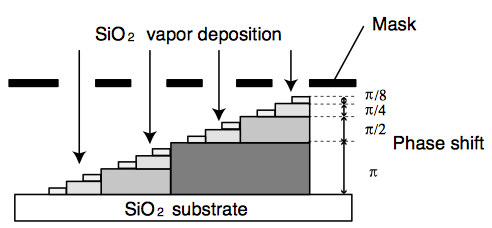
\includegraphics[scale=.5]{MSPP}
\caption{SiO$_2$ multilevel steps on a substrate.}
\label{mspp}
\end{figure}

\subsection*{Computer Generated Holography}
In CGH, an amplitude beam to be used as an optical vortex is directed through a hologram formed digitally and printed with extremely high resolution. The process for this formation is to incorporate both a planar wave used for reference, and the desired hologram obtained from an object wave. As these waves are combined, they for an interference pattern that can be printed and used as a filament for the optical vortex. When the beam propagates through this filament, there are an infinite number of diffraction orders produced with the first order beam containing the optical vortex. \cite{CGH}
\begin{figure}
\centering
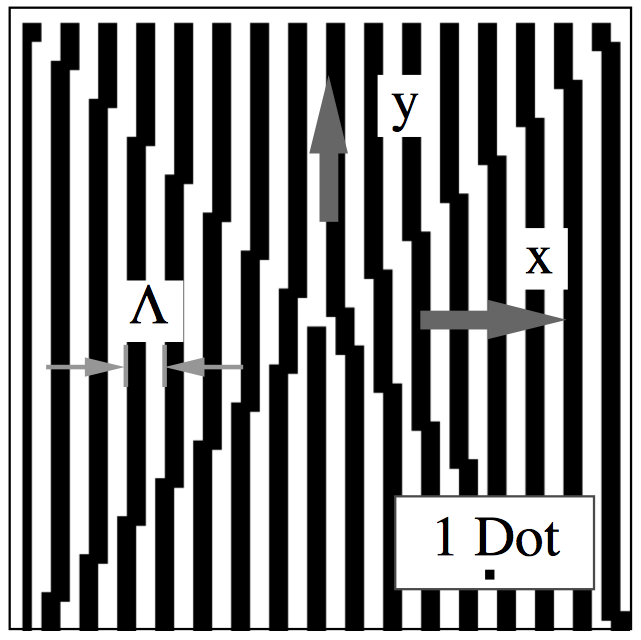
\includegraphics[scale=.2]{CGH.jpg}
\caption{Optical interference pattern.}
\label{}
\end{figure}


\newpage
\subsection*{Generation of Twisted Radio Waves}
Using a helical satellite dish, a team of physicists from Italy generated and sent a radio wave that corresponds to an $l=1$ helical vortex wave. 

\begin{figure}[h]
\centering
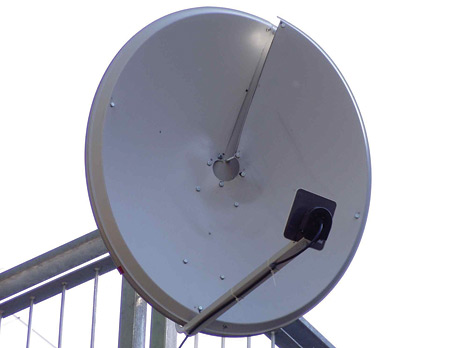
\includegraphics[scale=0.5]{helical_dish}
\caption{A helical dish used to transmit a twisted radio frequency.\cite{radio}}
\label{dish}
\end{figure}





%--------------Aaron's Application Section ---------------------------
\section*{Application: Producing and Detecting Non-interferring Othogonal Modes}
Using the 'twisted' radio waves produced by the helical dish and antenna in Fig. \ref{dish} and an untwisted radio wave, the team of physicists from Italy were able to transmit and receive two separate radio signals on the same frequency. These signals were crossed in space, and because of the orthogonal nature of the modes, did not interefere with each other. Other scientists have said in the past that it is not possible to produce these twisted radio signals far away from the dish (any further than the width of the dish), yet the group was able to transmit the signal across a significant distance (equal to more than 50 times the diamter of the dish). \\
\\
The Tamburini group uses the same profile equation equation ($u$) for their diverging electromagnetic wave. They used a $\sim$2.4 GHz radio transmission generated from two 2 Watt radio transmitters\cite{radio}. The main difference between the experiment performed and the calculations included in this report is that the topological charge $l$ is 1 in their experiment and $l=3$ for the calculations included. A radio transmitter can be made to fit the helicity of our topilogical charge.






\titlespacing{\section}{0pt}{\psl}{0pt}
\section*{Helical Modes of Light (Optical Vortices)}


The vector potential for a helical light beam traveling in the $\uv z$
and polarized in the $\uv x$ directions takes the form:
\begin{align*}
  \v A\p{r,\phi,z}&=A_0\f{w_0}{w}\sp{\f{r\sqrt 2}{w}}^\ell
  L^{\p{\ell}}_p\sp{2\f{r^2}{w^2}}\exp\sp{-\f{r^2}{w^2}}
  \exp\sp{-i\f{kr^2z}{2\p{z^2+z_R^2}}} \\
  &~~~~\times\exp\sp{i\p{2p+\ell+1}\arctan\p{\f z{z_R}}}
  \exp\p{i\ell\phi}\exp\p{-i\omega t} \uv x
\end{align*}
Here $A_0$ is a scaling factor, $w_0$ is the minimum beam waist, $w$
is the beam waist at the position $z$, $L^{\p{\ell}}_p$ is a
generalized Laguerre polynomial, $k$ is the wave vector, $\omega$ is
the frequency, $z_R$ is the Rayleigh length, $\ell$ is the topological
charge, and $p$ is the radial index. Parameters are given as follows:
\begin{align*}
  w=w_0\sqrt{1+z^2/z_R^2}
\end{align*}
\begin{align*}
  L^{\p{\ell}}_p\p{x}
  =\sum_{m=0}^p\p{-1}^m\f{\p{p+\ell}!}{\p{p-m}!\p{\ell+m}!m!}x^m
\end{align*}
\begin{align*}
  z_R=\f12 kw_0^2
\end{align*}
In particular, for $\p{\ell,p}=\p{3,1}$:
\begin{align*}
  L^{\p{3}}_1\p{x}=-x+4
\end{align*}
In the Coulomb gauge, we have $\del V=0$; for mutually perpendicular
$\v E$, $\v B$, and $\v k$ we must also have $\v k=k\uv z$. We can
then get the following electric ($\v E$) and magnetic ($\v B$) fields
from the complex vector potential $\v A_I$:
\begin{align*}
  \v E=i\omega\v A &&& \v B=-\del \times\v A
\end{align*}

The energy density $u$ is given by:
\begin{align*}
  u=\f12\p{\epsilon E^2+B^2/\mu}
\end{align*}

The Poynting vector $\v S$ is given by:
\begin{align*}
  \v S&=\v E\times\v B/\mu
\end{align*}

Beam intensity $I$ is given by:
\begin{align*}
  I=\f{c\epsilon}2E^2=\f c2\epsilon\omega^2A_I^2=cu/2
\end{align*}

The Maxwell stress tensor $\sigma_{ij}$ in our case is given by:
\begin{align*}
  \sigma_{ij}=\epsilon\p{E_iE_j-\f12\delta_{ij}E^2}
  +\f1\mu\p{B_iB_j-\f12\delta_{ij}B^2} =\delta_{ij}\f12\p{\epsilon
    E^2+B^2/\mu}=\delta_{ij}u
\end{align*}

The force per unit volume $\v f=f_i\uv e_i$ on matter is in turn:
\begin{align*}
  f_i=\d_k\sigma_{ik}-\d_tS_i/c^2=\d_iu-\delta_{iz}\d_tu/c
\end{align*}





\section*{Plotting the Results}

\begin{figure}[h]
\centering
\includegraphics[scale=0.4]{Ex-z-0-t-0}
\caption{$\hat{x}$ component of the calculated electric field.}
\label{g:Ex}
\end{figure}


\begin{figure}[h]
\centering
\includegraphics[scale=0.4]{By-z-0-t-0}
\includegraphics[scale=0.4]{Bz-z-0-t-0}
\caption{$\hat{y}$ and $\hat{z}$  component of the calculated magnetic field field.}
\label{g:By}
\end{figure}









\begin{figure}[h]
\centering
\includegraphics[scale=0.4]{Sy-z-0-t-0}
\includegraphics[scale=0.4]{Sz-z-0-t-0}
\caption{$\hat{y}$ and $\hat{z}$ component of the calculated electric field.}
\label{g:Sy}
\end{figure}


\begin{figure}[h]
\centering
\includegraphics[scale=0.4]{fmag-z-0-t-0}
\includegraphics[scale=0.4]{fx-z-0-t-0}
\includegraphics[scale=0.4]{fy-z-0-t-0}
\includegraphics[scale=0.4]{fz-z-0-t-0}
\caption{(Left to right, top to bottom) Magnitude, $\hat{x}$, $\hat{y}$ and $\hat{z}$ components of the calculated force per unit volume.}
\label{g:F}
\end{figure}



\begin{figure}[h]
\centering
\includegraphics[scale=0.4]{u-z-0-t-0}
\caption{Energy density $U$ of the electromagnetic wave, which is proportional to the intensity $I$ of the wave}
\label{g:F}
\end{figure}



\section*{Statement of Contribution}
\textbf{David --} Early research \\
\textbf{Grant --} Generation of vortex summary \\
\textbf{Aaron --} Application of vortex summary \\
\textbf{Michael --} Derivation of plotted quantities \\
\textbf{Paho --} Plotting\\

\bibliographystyle{IEEEtran} 
\bstctlcite{BSTcontrol}
\bibliography{optvort}

\end{document}